%----以下文字の大きさ,フォント,余白などを決定する設定----
\documentclass[a4paper,10pt]{jsarticle}
\setlength{\topmargin}{-17truemm}
\setlength{\oddsidemargin}{-0.4truemm}
\setlength{\textwidth}{160truemm}
\setlength{\textheight}{247truemm}
%-------------------------------------------------
%コンパイル方法 platex hoge.tex → platex hoge.tex → dvipdfmx hoge(サブファイルでも実行可能※ただし,サブファイルでコンパイルすると「他のサブファイルで定義された」ラベルを参照した時に?になる)
%bibtex適用のコンパイル platex hoge.tex → pbibtex hoge.tex → platex hoge.tex → platex hoge.tex → dvipdfmx hoge(メインファイルでのみ実行可能※サブファイルではコンパイルエラーが起きる)
%\usepackage{}:Latexで拡張機能を使用するための宣言-------------
\usepackage[dvipdfmx]{graphicx}%図を埋め込むためのパッケージ
\usepackage{float}%その場に表・図を表示させるパッケージ

\usepackage[dvipdfmx]{hyperref}%しおり作成のためのパッケージ
\usepackage{pxjahyper}%しおりを日本語化

\title{タイトル}%タイトル
\author{田中太郎}%著者
\date{2000年1月1日}%日付

\begin{document}%本文の始まり
\maketitle%上記で設定したtitle,author,dateを表示

\section{図}
図\ref{fig:hoge}を参照します.
\begin{figure}[H]
    \begin{center}
        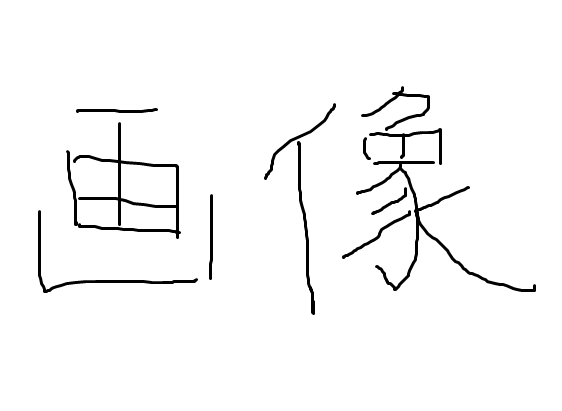
\includegraphics[width=120mm]{fig/image1.png}
    \end{center}
    \caption{hoge}
    \label{fig:hoge}
\end{figure}

\end{document}

%-------ラベル,参照----------
%\label{fig:hoge}

%図--------------------
%\begin{figure}[H]
%    \begin{center}
%        \includegraphics[width=120mm]{\PATH/fig/hoge.eps}
%    \end{center}
%    \caption{hoge}
%    \label{fig:hoge}
%\end{figure}